\chapter{Newtonian Gravity, Gauss's Law, and the Equivalence Principle}

These notes follow Leonard Susskind's second lecture on general relativity in the order in which the argument is actually built. The lecture opens with a short detour about dark energy, then deliberately returns to Newtonian gravity, sharpens that old physics into field language, and only then turns toward Einstein. Where the blackboard itself carries part of the mathematical story, we keep the original lecture frames visible as documentary evidence and place the cleaned equations or diagrams nearby. Credit for the lecture belongs to Leonard Susskind; the present curation also owes explicit credit to LazyingArt LLC and Video2Book.

\section{Dark Energy as a Prelude, Not the Main Road}

The lecture begins by answering a worry that had been left hanging over from earlier exchanges: if dark energy acts like a repulsive component of gravity, why does it not tear ordinary bound systems apart? Susskind does not begin with cosmological field equations. He begins with a spring, because for the limited point he wants to make, that is the cleanest picture.

For an ordinary restoring force we may write, schematically,
\begin{equation}
F(r)\sim -kr.
\end{equation}
A positive cosmological constant is then modeled, at this opening level, as a tiny repulsive correction of the same distance-dependent type,
\begin{equation}
F(r)\sim -kr+\lambda r.
\end{equation}
The point is not that an atom literally is a spring. The point is that if a bound system already has a strong restoring force, then a very small repulsive term proportional to distance merely shifts the equilibrium position slightly. It weakens the binding a little; it does not destroy it.

That is the practical content of the opening discussion. The coefficient $\lambda$ is so small that its effect is negligible on laboratory scales, negligible on the scale of the solar system, and still tiny compared with ordinary binding effects inside galaxies. Only on cosmological scales does such a term compete with anything else.

Susskind then sharpens the contrast by mentioning the ``Big Rip'' scenario. The ordinary cosmological constant does not do this. The rip would require something more violent: effectively, that the repulsive coefficient grow with time. He treats that not as sober mainstream physics, but as a bad speculative idea.

\subsection{Question \& Answer}

\paragraph{Question.} Why does dark energy not tear atoms, solar systems, or galaxies apart?

\paragraph{Answer.} Because in the lecture's opening model the repulsive contribution is fantastically small. In a bound system it produces, to leading order, only a slight shift of the equilibrium configuration. The atom becomes a tiny bit larger; the orbit becomes a tiny bit more spread out. The ``Big Rip'' picture would require the repulsive effect to grow with time and eventually overwhelm binding forces. Susskind explicitly treats that as a different and much less credible story.

With the conceptual debris cleared away, the lecture returns to where it meant to go all along: we still need a little more Newton before we can earn Einstein.

\section{A Little Formalism: Del, Fields, and the Gravitational Acceleration}

Susskind introduces this next step with exactly the right tone: first a little mathematics, though really it is only formalism, a notation for organizing equations. The operator
\begin{equation}
\nabla = (\partial_x,\partial_y,\partial_z)
\end{equation}
behaves symbolically like a vector, even though it is really a differential operator.

If $\phi(x,y,z)$ is a scalar field, then applying $\nabla$ produces a vector field,
\begin{equation}
\nabla \phi
=
\left(
\partial_x\phi,\,
\partial_y\phi,\,
\partial_z\phi
\right).
\end{equation}
If instead $\vec v(x,y,z)$ is a vector field, then the divergence is the scalar
\begin{equation}
\nabla\cdot\vec v
=
\partial_x v_x+\partial_y v_y+\partial_z v_z.
\end{equation}
We should keep the bookkeeping completely straight here. The lecture contains a fleeting verbal slip, but the mathematics is unambiguous: the gradient of a scalar is a vector, while the divergence of a vector is a scalar.

A scalar field is just a scalar quantity depending on position. A vector field is a vector quantity depending on position. The Newtonian gravitational field is such a vector field.

Now Susskind defines it operationally. Take a distribution of source masses $m_i$ at positions $\vec x_i$. Introduce a tiny test mass, release it at the field point $\vec x$, and observe its acceleration. That acceleration is the gravitational field:
\begin{equation}
\vec A(\vec x)=\text{acceleration of a test mass released at }\vec x.
\end{equation}
There is a brief and telling hesitation over the sign convention. That hesitation should not be erased, because it shows exactly what must be fixed. We want the field to point \emph{toward} the source mass. Therefore we choose
\begin{equation}
\vec R_i := \vec x_i-\vec x,
\end{equation}
so that $\vec R_i$ points from the test mass toward the $i$th source. With that choice the Newtonian field is
\begin{equation}
\vec A(\vec x)
=
G\sum_i m_i \frac{\vec R_i}{R_i^3}
=
G\sum_i m_i \frac{\hat R_i}{R_i^2},
\qquad
\hat R_i=\frac{\vec R_i}{R_i}.
\end{equation}
That is simply the inverse-square law rewritten as a field at a point. The magnitude scales like $1/R_i^2$; the direction is carried by $\vec R_i$.

\begin{figure}[ht]
\centering

\includegraphics[width=.62\textwidth]{lecture_02_figure_02.png}

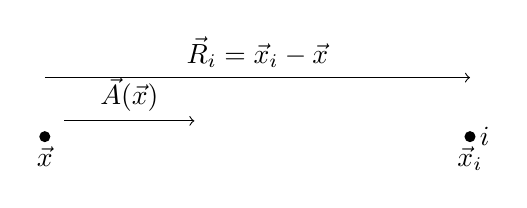
\begin{tikzpicture}[scale=1.0]
\fill (0,0) circle (2pt);
\fill (5.4,0) circle (2pt);
\node[below] at (0,0) {$\vec x$};
\node[below] at (5.4,0) {$\vec x_i$};
\node[right] at (5.4,0) {$i$};
\draw[->] (0,0.75) -- (5.4,0.75) node[midway, above] {$\vec R_i=\vec x_i-\vec x$};
\draw[->] (0.25,0.2) -- (1.9,0.2) node[midway, above] {$\vec A(\vec x)$};
\end{tikzpicture}
\caption{Field vector and source-point displacement. The board frame is kept because it is the clearest documentary evidence for the source-point/field-point geometry, while the redraw fixes the final sign convention chosen in the lecture.}
\end{figure}

Up to this point the field has been assembled one source at a time. The next move is the one Susskind explicitly advertises: there is a neat way to summarize all this.

\section{Gauss's Law as Physics, Gauss's Theorem as Mathematics}

To pass from discrete particles to a field equation, we introduce the mass density. If a small volume $\Delta V$ contains a small mass $\Delta m$, then
\begin{equation}
\rho = \frac{\Delta m}{\Delta V}.
\end{equation}
In the continuum picture $\rho(\vec x)$ is itself a scalar field.

Now comes the summary of Newtonian gravity:
\begin{equation}
\nabla\cdot\vec A = -4\pi G\rho.
\end{equation}
This is Gauss's law for gravity. The minus sign records the fact that the field points inward toward positive mass. The field converges. A convergence is a negative divergence.

Susskind is especially careful here to separate two statements that are often blurred together. Gauss's law is physics. It is a law of nature, equivalent to Newtonian gravity. Gauss's theorem is mathematics. It says that for any sufficiently nice region $V$ with boundary $\partial V$,
\begin{equation}
\int_V (\nabla\cdot\vec A)\,dV
=
\oint_{\partial V} A_\perp\,d\sigma.
\end{equation}
On the left we integrate the divergence throughout the volume. On the right we integrate the component of the field normal to the boundary. The theorem translates volume divergence into boundary flux.

The blackboard frame for this moment is only partially legible, but the intent is clear enough to justify writing the standard form.

\begin{figure}[ht]
\centering

\includegraphics[width=.58\textwidth]{lecture_02_figure_03.png}

\begin{tikzpicture}[scale=1.0]
\draw (-2.4,-1.2) .. controls (-2.9,0.5) and (-1.4,1.8) .. (0.2,1.3)
.. controls (1.6,0.9) and (2.3,-0.1) .. (1.4,-1.2)
.. controls (0.2,-1.8) and (-1.4,-1.9) .. (-2.4,-1.2);
\draw (1.55,0.15) -- (2.15,0.15) -- (2.15,0.78) -- (1.55,0.78) -- cycle;
\draw[->] (1.85,0.46) -- (3.0,0.46);
\node[right] at (3.0,0.46) {$A_\perp$};
\node[above] at (1.85,0.78) {$d\sigma$};
\end{tikzpicture}
\caption{Surface-flux term in Gauss's theorem. The lecture frame shows the half-written theorem and the boundary patch labeled $A_\perp$; the redraw makes explicit that the theorem uses the normal component through the surface element $d\sigma$.}
\end{figure}

This is still abstract. The lecture does not linger there. Susskind immediately says, in effect, let us put them together and see what they do.

\section{Putting Them Together: Exterior Fields and the Shell Theorem}

Suppose the mass distribution is spherically symmetric, or isotropic, about a center. Then we surround it by a concentric Gaussian sphere of radius $r$. Now the theorem and the law meet each other.

From Gauss's law,
\begin{equation}
\nabla\cdot\vec A = -4\pi G\rho,
\end{equation}
so inside the volume integral we have
\begin{equation}
\int_V (\nabla\cdot\vec A)\,dV
=
-4\pi G\int_V \rho\,dV.
\end{equation}
But the integral of $\rho$ over the volume is simply the enclosed mass,
\begin{equation}
\int_V \rho\,dV = M_{\mathrm{enc}}.
\end{equation}
Meanwhile, on the surface side, symmetry tells us something equally important. The field must be radial, and its radial component has the same value at every point of the Gaussian sphere. Therefore
\begin{equation}
\oint_{\partial V} A_\perp\,d\sigma = 4\pi r^2 A_r.
\end{equation}
Putting these together gives
\begin{equation}
4\pi r^2 A_r = -4\pi G M_{\mathrm{enc}},
\end{equation}
and therefore
\begin{equation}
A_r = -\frac{G M_{\mathrm{enc}}}{r^2}.
\end{equation}
If the sphere encloses the whole body, then $M_{\mathrm{enc}}=M$, and we recover the familiar inverse-square field
\begin{equation}
A_r = -\frac{GM}{r^2}.
\end{equation}

This is also the point in the lecture where Susskind remarks on the appearance of the factor $4\pi$. In this normalization it is chosen so that the surface area of the sphere cancels cleanly. One could normalize the equations differently, but this choice makes spherical problems fall open at once.

\begin{figure}[ht]
\centering

\includegraphics[width=.62\textwidth]{lecture_02_figure_04.png}

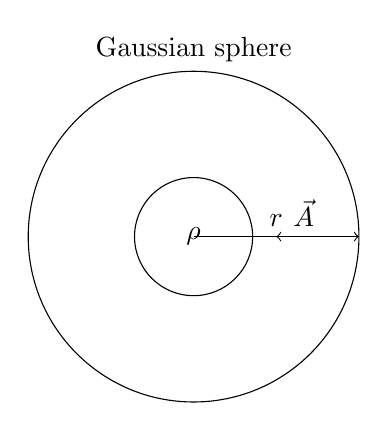
\begin{tikzpicture}[scale=1.0]
\draw (0,0) circle (2.1);
\draw (0,0) circle (0.75);
\draw[->] (0,0) -- (2.1,0) node[midway, above] {$r$};
\draw[->] (1.75,0) -- (1.05,0) node[midway, above] {$\vec A$};
\node at (0,0) {$\rho$};
\node[above] at (0,2.1) {Gaussian sphere};
\end{tikzpicture}
\caption{Gauss law with enclosed mass. The lecture frame shows the shift from the abstract flux theorem to the gravitational mass integral; the redraw isolates the concentric spherical geometry used in the derivation.}
\end{figure}

What has happened is more than a recovery of Newton's formula. We have also learned something new in this language: the exterior field of any spherically symmetric mass distribution is the same as the field of a point mass at the center.

\subsection{Question \& Answer}

\paragraph{Question.} Why does only the mass inside the Gaussian sphere matter?

\paragraph{Answer.} Because the flux through the Gaussian sphere is fixed by the integral of the density \emph{inside} that sphere. Once spherical symmetry is assumed, the flux determines the radial field on the boundary. Matter outside contributes zero net field there. This is the shell theorem in flux form.

That answer has a remarkable corollary. If the entire mass were placed on a thin spherical shell, then the field inside the shell would vanish identically. Outside, the field would be exactly the same as that of a point mass at the center. Susskind emphasizes that Newton knew this and proved it geometrically, without calculus. In these notes we see it fall directly out of Gauss's law.

\section{While We Are At It: Inside the Earth}

At this point Susskind turns, in the same spirit, to a question from the previous meeting: what does the gravitational field look like \emph{inside} the Earth? The same formalism answers it almost for free.

We again choose a Gaussian sphere, but now the sphere lies inside the Earth. The flux side is unchanged:
\begin{equation}
\oint_{\partial V} A_\perp\,d\sigma = 4\pi r^2 A_r,
\end{equation}
where $r$ is now the radius of the \emph{inner} Gaussian sphere. What changes is the mass enclosed.

To make the calculation explicit, Susskind adopts a simplified Earth: uniform density $\rho$ throughout the interior, abruptly dropping to zero at the surface. Then
\begin{equation}
M_{\mathrm{enc}}(r)=\frac{4\pi}{3}r^3\rho.
\end{equation}
Substituting this into Gauss's law gives
\begin{align}
4\pi r^2 A_r
&=
-4\pi G M_{\mathrm{enc}}(r),\\
4\pi r^2 A_r
&=
-4\pi G\left(\frac{4\pi}{3}r^3\rho\right).
\end{align}
The board algebra in the lecture becomes momentarily unstable here, and the audience catches a missing factor of $4\pi$. The corrected result, which is the one we should preserve, is
\begin{equation}
A_r = -\frac{4\pi G\rho}{3}\,r.
\end{equation}
This also matches the exterior formula at the surface $r=R$ once we use
\begin{equation}
M=\frac{4\pi}{3}R^3\rho.
\end{equation}

\begin{figure}[ht]
\centering

\includegraphics[width=.62\textwidth]{lecture_02_figure_05.png}

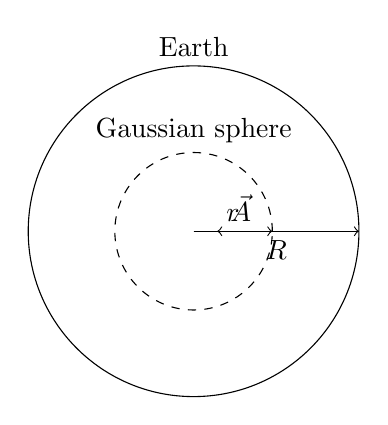
\begin{tikzpicture}[scale=1.0]
\draw (0,0) circle (2.1);
\draw[dashed] (0,0) circle (1.0);
\draw[->] (0,0) -- (1.0,0) node[midway, above] {$r$};
\draw[->] (0,0) -- (2.1,0) node[midway, below] {$R$};
\node[above] at (0,2.1) {Earth};
\node[above] at (0,1.0) {Gaussian sphere};
\draw[->] (0.9,0) -- (0.3,0) node[midway, above] {$\vec A$};
\end{tikzpicture}
\caption{Concentric spheres and enclosed-mass factor. The preserved lecture frame supplies the documentary evidence for the inner Gaussian sphere and the visible $\frac{4\pi}{3}r^3\rho$ factor, while the redraw gives the cleaned geometry for the corrected derivation.}
\end{figure}

Now the lecture cashes out the result physically. Since $\vec A$ is an acceleration field, multiplying by the mass $m$ of the test particle gives
\begin{equation}
m\ddot r = -\frac{4\pi G\rho}{3}\,mr.
\end{equation}
This is the equation of a harmonic oscillator. Inside the idealized uniform Earth, gravity becomes a linear restoring force.

That is a lovely Newtonian payoff. A particle displaced from the center is pulled back exactly as though attached to a spring. In the tunnel-through-the-Earth thought experiment, the particle would oscillate through the planet.

\subsection{Question \& Answer}

\paragraph{Question.} How can the field be linear in $r$ if the enclosed mass grows like $r^3$?

\paragraph{Answer.} Because Gauss's law fixes the \emph{flux}, not the field directly. The flux contains an area factor $4\pi r^2$. Thus the scaling is
\begin{equation}
A_r \, r^2 \sim r^3,
\end{equation}
so only one power of $r$ survives:
\begin{equation}
A_r \sim r.
\end{equation}
This is exactly the local conceptual snag that surfaces in the classroom, and it is useful because it makes visible the role of the Gaussian sphere itself.

The lecture briefly announces gravitational potential here, but then defers it. That deferral is important. The Newtonian recap has reached the point it needed to reach, and Susskind is ready to say so: this has been old physics. Now we move to the new idea.

\section{The Equivalence Principle as Elevator Intuition and Coordinate Transformation}

The equivalence principle first appears in the lecture in the form everybody remembers: the elevator. Suppose we have a cabin accelerating horizontally with acceleration $g$. A passenger releases an object inside. In the inertial frame outside the elevator, the object simply continues its motion. But to the observer riding inside, the object accelerates backward toward the floor of the elevator with magnitude $g$. It looks like gravity, sounds like gravity, smells like gravity.

Susskind insists that this alone would not make Einstein Einstein. The real step is not merely to say the words. The real step is to use them. But before he uses them, he rebuilds the elevator mathematically.

\begin{figure}[ht]
\centering
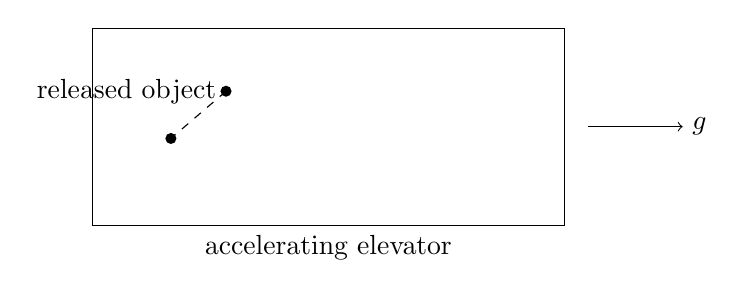
\begin{tikzpicture}[scale=1.0]
\draw (0,0) rectangle (6,2.5);
\draw[->] (6.3,1.25) -- (7.5,1.25) node[right] {$g$};
\fill (1.7,1.7) circle (2pt);
\draw[dashed] (1.7,1.7) -- (1.0,1.1);
\fill (1.0,1.1) circle (2pt);
\node[below] at (3,0) {accelerating elevator};
\node[left] at (1.7,1.7) {released object};
\end{tikzpicture}
\caption{Horizontal elevator version of the equivalence principle. In the passenger's frame, the released object accelerates backward toward the floor exactly as if a uniform gravitational field were present.}
\end{figure}

He chooses the horizontal coordinate $x$ precisely because he wants to draw an $x$--$t$ diagram. First consider uniform velocity. If the floor of the elevator moves with constant speed $v$, then the passenger's coordinate relative to the floor is
\begin{equation}
x' = x-vt,
\qquad
t'=t.
\end{equation}
This is still Newtonian physics: all observers use the same time. If an object is at rest in the inertial frame, then $x=\text{constant}$ and hence
\begin{equation}
\dot x' = -v,
\qquad
\ddot x' = 0.
\end{equation}
So a uniformly moving frame creates no fictitious gravitational field.

Now let the elevator accelerate uniformly. Its floor then follows
\begin{equation}
x_{\mathrm{floor}}(t)=\frac{1}{2}gt^2,
\end{equation}
and the corresponding transformed coordinate is
\begin{equation}
x' = x-\frac{1}{2}gt^2.
\end{equation}
For an object at rest in the inertial frame, we differentiate once and then again:
\begin{equation}
\dot x' = -gt,
\qquad
\ddot x' = -g.
\end{equation}
This is the mathematical statement of the elevator argument. In the accelerated frame, freely moving bodies behave as though there were a uniform gravitational field.

\begin{figure}[ht]
\centering
\begin{tikzpicture}[scale=0.92]
\draw[->] (-0.2,0) -- (4.8,0) node[right] {$x$};
\draw[->] (0,-0.2) -- (0,4.8) node[above] {$t$};
\draw (0.8,0) -- (0.8,4.2);
\draw (2.2,0) -- (3.75,4.0);
\node at (0.8,4.45) {$x=\mathrm{const}$};
\node at (3.45,4.45) {$x'=0$};
\node at (2.3,-0.45) {uniform velocity};
\end{tikzpicture}

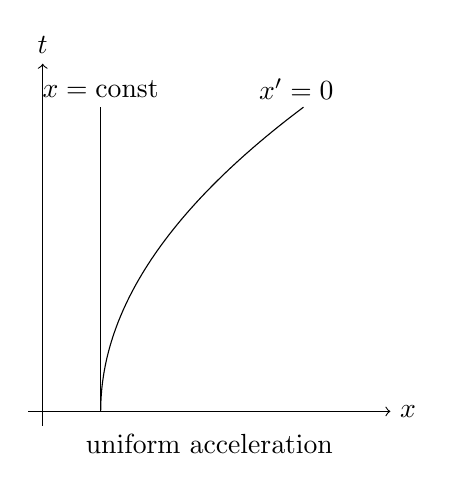
\begin{tikzpicture}[scale=0.92]
\draw[->] (-0.2,0) -- (4.8,0) node[right] {$x$};
\draw[->] (0,-0.2) -- (0,4.8) node[above] {$t$};
\draw (0.8,0) -- (0.8,4.2);
\draw plot[smooth,domain=0:2.0] ({0.8+0.7*\x*\x},{2.1*\x});
\node at (0.8,4.45) {$x=\mathrm{const}$};
\node at (3.5,4.45) {$x'=0$};
\node at (2.3,-0.45) {uniform acceleration};
\end{tikzpicture}
\caption{$x$--$t$ sketches for the moving and accelerating elevator. The accelerating floor follows a parabola, and the transformed coordinate produces the effective field $\ddot x'=-g$.}
\end{figure}

This is not yet full relativity. Susskind says so directly. But it already gives the conceptual bridge he wants: acceleration corresponds to a change to curvilinear coordinates in space-time. That is why the discussion is heading toward geometry.

\section{Einstein's Move: Light, Locality, and the Metric}

Now comes the genuinely Einsteinian use of the principle. If gravity and acceleration are equivalent only for falling stones, then the principle is not deep. Einstein's claim is stronger: the laws of physics in a gravitational field are the same as the laws of physics in an accelerated frame. Therefore the principle must apply to light as well.

Imagine an elevator standing still. A light beam sent horizontally across it travels in a straight line and hits the opposite wall directly across. Now imagine the elevator accelerating upward. The light beam still begins horizontally, but by the time it reaches the far wall the elevator has moved upward. So in the elevator frame the light lands lower than before. Its path is curved. In fact, in this approximation, it is parabolic.

\begin{figure}[ht]
\centering
\begin{tikzpicture}[scale=1.0]
\draw (0,0) rectangle (6,3.5);
\draw[->] (3,3.8) -- (3,4.8) node[above] {$g$};
\fill (0.6,2.7) circle (2pt);
\draw (0.6,2.7) .. controls (2.1,2.65) and (4.1,2.15) .. (5.25,1.2);
\draw[->] (0.6,2.7) -- (5.25,1.2);
\node[left] at (0.6,2.7) {light};
\node[right] at (5.25,1.2) {hit point};
\end{tikzpicture}
\caption{Light in an upward-accelerating elevator. This is the elevator version of the statement that light falls in a gravitational field.}
\end{figure}

That simple argument leads to Einstein's early estimate for light bending by the Sun. The lecture keeps the estimate rough and historical, and the notes should do the same. Consider a light ray that just skims the solar surface. Near closest approach, take the downward acceleration to be roughly the surface gravity,
\begin{equation}
g_\odot \approx \frac{GM}{R^2}.
\end{equation}
The time spent in the region where this matters is estimated by the light-crossing time of about two solar radii:
\begin{equation}
\Delta t \approx \frac{2R}{c}.
\end{equation}
Hence the downward component of the velocity picked up by the ray is
\begin{equation}
\Delta v_\perp \approx g_\odot \Delta t \approx \frac{2GM}{Rc}.
\end{equation}
For a small deflection angle,
\begin{equation}
\theta \approx \frac{\Delta v_\perp}{c}\approx \frac{2GM}{Rc^2}.
\end{equation}

\begin{figure}[ht]
\centering
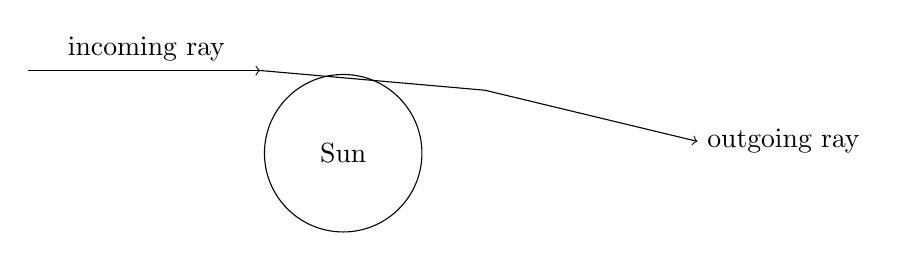
\begin{tikzpicture}[scale=1.0]
\draw (0,0) circle (1.0);
\node at (0,0) {Sun};
\draw[->] (-4,1.05) -- (-1.05,1.05);
\draw (-1.05,1.05) -- (1.8,0.8);
\draw[->] (1.8,0.8) -- (4.5,0.15);
\node[above] at (-2.5,1.05) {incoming ray};
\node[right] at (4.5,0.15) {outgoing ray};
\end{tikzpicture}
\caption{Crude sun-skimming-ray estimate. The lecture treats the deflection qualitatively and then estimates it by combining surface gravity with a light-crossing time.}
\end{figure}

This is Einstein before the full apparatus of general relativity. Susskind keeps the historical caution in view: the final relativistic answer differs by a factor of two. The point of the lecture here is not precision but the conceptual use of the equivalence principle in a place where nobody had used it before.

\subsection{Question \& Answer}

\paragraph{Question.} Can free fall completely eliminate gravity, or only locally?

\paragraph{Answer.} Only locally. A sufficiently small elevator, observed for a sufficiently short time, can replace the Earth's field by a single accelerating frame. But the real Earth's field is not uniform. Its direction varies from place to place, and its magnitude varies with distance. A large enough freely falling body notices this immediately: its feet are pulled more strongly than its head, and neighboring free-fall lines converge sideways. Those are tidal forces. They are the obstruction to eliminating gravity globally.

That is the limiting correction Susskind insists on before the lecture ends. Gravity can be transformed away only in a local neighborhood. The real, invariant content of a gravitational field lies in what survives that attempt, namely tidal effects.

He then steps back from mechanics and turns to the blackboard itself. How does one describe the geometry of a flat two-dimensional surface? In rectangular Cartesian coordinates, for neighboring points,
\begin{equation}
ds^2 = dx^2 + dy^2.
\end{equation}
But in curvilinear coordinates on the same flat board, the distance between neighboring points is more generally
\begin{equation}
ds^2 = g_{xx}\,dx^2 + 2g_{xy}\,dx\,dy + g_{yy}\,dy^2.
\end{equation}
The cross term tells us that the coordinate lines need not be perpendicular. The position dependence of the coefficients tells us that the coordinate mesh can stretch, squeeze, and twist from place to place. These functions are the metric.

Now the final bridge of the lecture can be stated cleanly. Curvature is the obstruction to finding coordinates that globally flatten the geometry. Tidal forces are the obstruction to finding coordinates that globally eliminate the gravitational field. The connection is not accidental. It is the first glimpse of general relativity as geometry.

\section{Summary}

Lecture 2 begins with a seemingly peripheral question about dark energy, but that opening detour performs useful work: it clears away confusion before the main argument returns to Newton. The Newtonian part of the lecture is then rebuilt in a more modern field language. We define the gravitational field as the acceleration of a test mass, summarize the many-body inverse-square law by
\[
\nabla\cdot\vec A = -4\pi G\rho,
\]
and combine Gauss's law with Gauss's theorem to recover both the exterior inverse-square field and the linear interior field of a uniform-density Earth.

Only after that long Newtonian runway does Einstein's idea become sharp. An accelerated elevator produces an effective gravitational field; the transformed coordinate satisfies $\ddot x'=-g$; and once one takes that principle seriously for all physics, light itself must bend. But the principle is only local. Tidal forces remain. That is why the lecture ends with the metric and curvature: not yet with the full theory, but with the right obstruction, the right bridge, and the right sense that gravity is what cannot finally be transformed away.